\documentclass[tikz,border=10pt]{standalone}
% No extra TikZ libraries needed.
\begin{document}
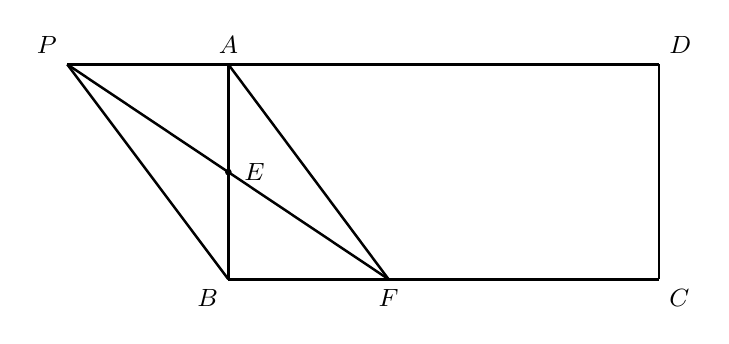
\begin{tikzpicture}[line width=0.9pt, line join=round,
  every node/.style={font=\fontsize{9}{10.8}\selectfont}]
  % Points: origin at P, s = 0.011561 cm per px, y flipped
  \coordinate (P) at (0,0);
  \coordinate (A) at (2.046,0);
  \coordinate (D) at (7.515,0);
  \coordinate (B) at (2.046,-2.729);
  \coordinate (C) at (7.515,-2.729);
  \coordinate (F) at (4.081,-2.729);
  % E = PF ∩ AB, at px (224,184.33): y = -(184.33-66)*0.011561
  \coordinate (E) at (2.046,-1.368);

  % Segments (solid, black)
  \draw (P) -- (D);          % top horizontal P-A-D
  \draw (B) -- (C);          % bottom horizontal B-F-C
  \draw (A) -- (B);          % vertical A-B
  \draw (D) -- (C);          % vertical D-C
  \draw (P) -- (F);          % diagonal P-F
  \draw (A) -- (F);          % diagonal A-F
  \draw (P) -- (B);          % diagonal P-B

  % Labels outside each vertex
  \node[above left] at (P) {$P$};
  \node[above] at (A) {$A$};
  \node[above right] at (D) {$D$};
  \node[below left] at (B) {$B$};
  \node[below right] at (C) {$C$};
  \node[below] at (F) {$F$};

  % Intersection point E on AB
  \fill (E) circle (1.2pt);
  \node[right=2pt] at (E) {$E$};
\end{tikzpicture}
\end{document}